\chapter{Selective Velocity Obstacle}
\label{Ch:IntroductionSVOI}

%thisw part is From JGCD01 - SVO for Cooperative

\section{Introduction}
\lettrine[lines=3, nindent=0pt]{C}{urrently}, Unmanned Aerial Vehicle (UAV) technology is advancing into everyday applications and, as a result, concern has arisen on the safety of their operations in the civil airspace\cite{Dalamagkidis:09}. One of the main problems is the autonomous avoidance of mid-air collisions with other UAVs, which has driven many studies to develop various algorithms for a collision avoidance system. 

For civil UAV avoidance, the Geometric Guidance algorithms are potentially best suited since they do not need to conduct extensive predictions and analyses, which require large computational resources on-board. Instead, they give solutions reactively based on the instantaneous geometry of an imminent conflict. Examples of Geometric Guidance include the Collision Cone\cite{Chakravarthy:98,Lorenz:13}, the Velocity Obstacle Method (VO-method)\cite{Fiorini:98,Kluge:06,vdberg:08,Snape:11,Choi:13,Ellerbroek2013c}, the Minimum Effort Guidance (MEG)\cite{Watanabe:13}, and the Differential Geometric Guidance\cite{Mujumdar:12}. 

Most of those studies, however, neglect the situation in a controlled airspace where the UAVs are heterogeneous, each with its own mission and preference for avoidance. Furthermore, there might be various procedures and rules enforced by the authorities to manage the airspace. Several existing methods that consider those kinds of situations are commonly predictive methods, for instance the Airborne Collision Avoidance System X (ACAS X)\cite{kochenderfer:2012}, or the Jointly Optimal Conflict Avoidance (JOCA)\cite{Graham:11}.

This paper proposes a novel method for UAV-to-UAV autonomous collision avoidance called the Selective Velocity Obstacle method (SVO). The method is an extension of the former Velocity Obstacle method\cite{Fiorini:98} that is designed to reactively generate an avoidance maneuver based on conflict geometry. The maneuver generated from the SVO is a deconflict maneuver, a tactical maneuver that aims to avoid obstacles while limiting the deviation from the original route. Following the avoidance system architecture presented in Ref.\cite{barfield:00} and \cite{Jenie:13a}, the maneuver can start anywhere within a particular zone called the deconflict-zone, as shown in figure~\ref{f:Architecture}. The zones in the figure can also represent the layers of safety that use deconflict maneuvers in the architecture presented in Ref.\cite{Jenie:15}. The conflict cases for SVO are set to be heterogeneous, involving vehicles with different characteristics and missions. To comply with the vision of the European Commission for Unmanned Aerial System (UAS)\cite{INOUI}, all of the avoidance in SVO is implicitly coordinated by incorporating the right-of-way rules\cite{FAR:91}, which also reduce the complexity of solution for heterogeneous conflicts.

\begin{figure}[h]
\centering
 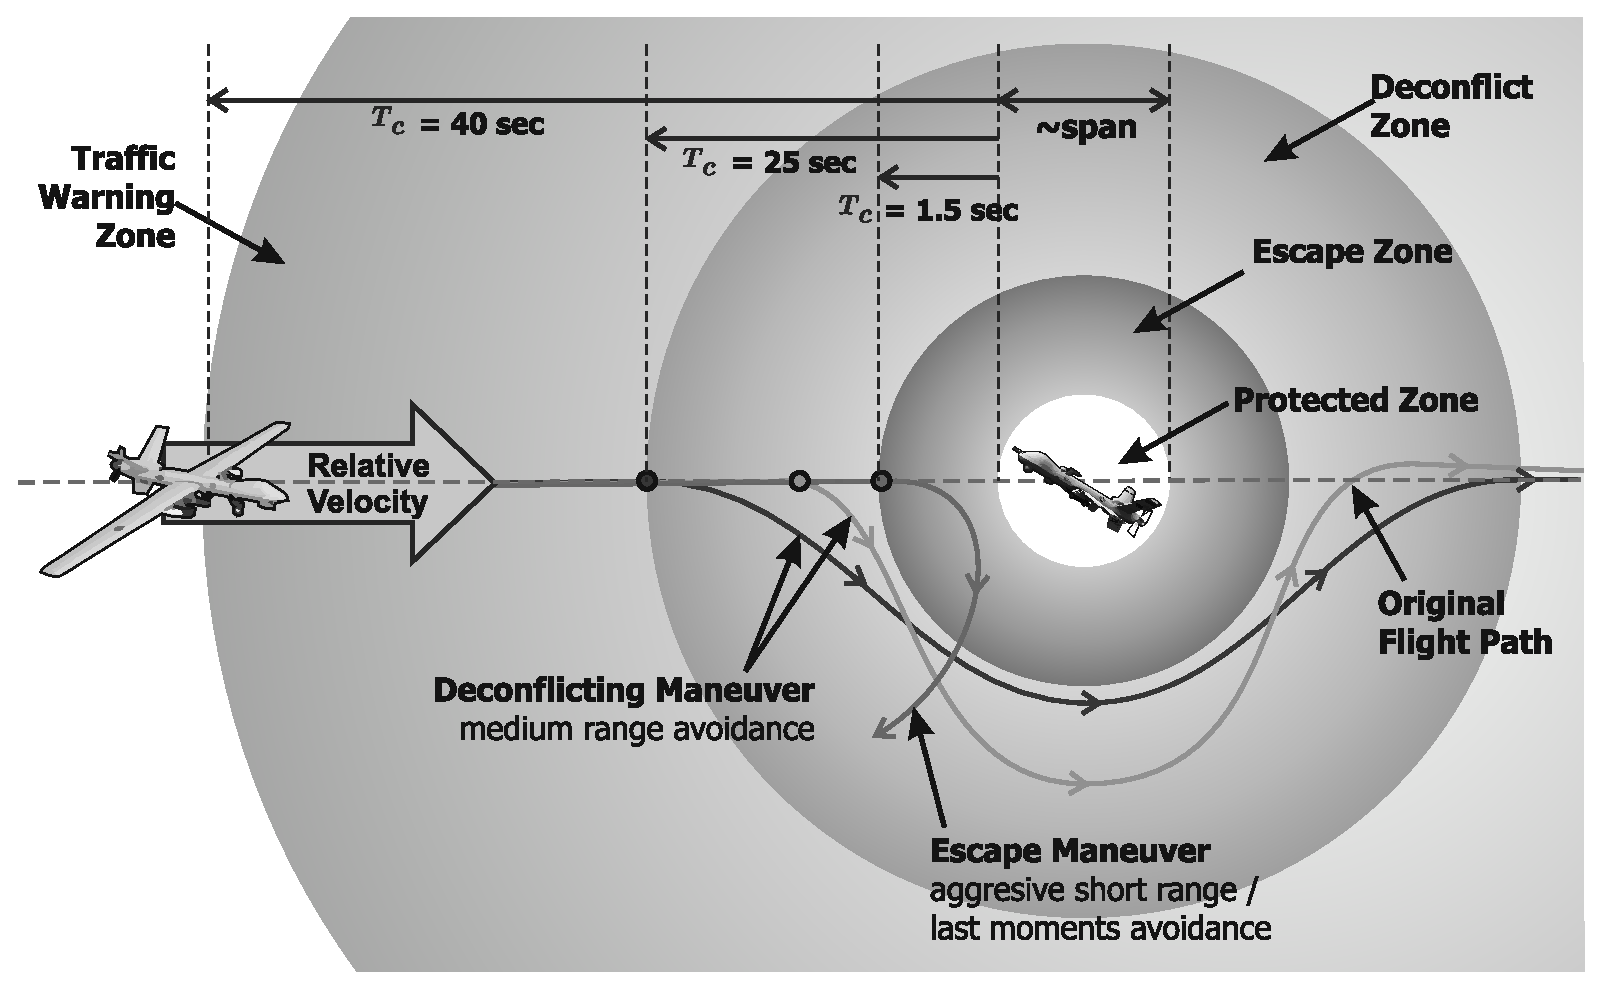
\includegraphics[width=8cm]{\TheDir Figures/AvoidanceStructure}
 \caption{Architecture of collision avoidance for UAVs, adapted from Ref.\cite{barfield:00} and  \cite{Jenie:13a}.}
 \label{f:Architecture}
\end{figure}

Elaborated in Section II, the conflict situations in the airspace, which includes the heterogeneousness and the rules based coordination, are modeled in the Velocity Obstacle framework. A few problems in the previous method are identified and solved throughout this section. Several simulations are presented in Section III to demonstrate the performance of the method, along with a validation using Monte Carlo simulations. This is then followed by the conclusions in Section IV.

\section{Selective Velocity Obstacle Method for UAV Collision Avoidance}

Figure~\ref{f:OVOconcept} shows an example of a two-dimensional encounter situation between two UAVs, referred to as the own-ship and the obstacle. The own-ship must first decide whether or not a situation is a conflict and, if necessary, conduct any appropriate resolution maneuver. In this case, the conflict is defined when the own-ship violates the escape-zone, $S_{esc}$, a circle with radius of $r_{esc}$ from the center of the obstacle.

%[figure 3]
\begin{figure}[h]
\centering
 \includegraphics[width=8cm]{\TheDir Figures/OVOconcept}
 \caption{Velocity-obstacle set generation from an instantaneous encounter situation, adapted from Ref.\cite{Fiorini:98}.}
 \label{f:OVOconcept}
\end{figure}

\subsection{Original Concept of the Velocity Obstacle Method}
The concept of the original Velocity Obstacle method (OVO) presented in this section is adapted from Ref.~\cite{Fiorini:98}. In figure~\ref{f:OVOconcept}, the Collision-cone, $CC_{oi}$, is generated from an instantaneous situation by collecting relative velocity extensions, $\lambda_{V_R}$, that cut through the $S_{esc}$. The Velocity Obstacle set, $VO_{oi}$, is the translation of the $CC_{oi}$ along the shadow of the obstacle velocity, $V_i'$. The OVO uses this $VO_{oi}$ set to determine the conflict: The own-ship will violate the $S_{esc}$ at some time in the future if and only if $V_o \in VO_{oi}$. The method also determines whether the two vehicles are diverging or not, with the use of the diverging set, $DIV_{oi}$: The own-ship is diverging the obstacle if and only if $V_o \in DIV_{oi}$. The two determinations are made under the assumption that both velocities $V_o$ and $V_i$ are constant.

An avoidance maneuver is conducted whenever $V_o \in VO_{oi}$, by updating the $V_o$ to a new velocity that is outside the $VO_{oi}$ set. The common strategy is to choose the closest point from the current $V_o$ on one of the $VO_{oi}$ edges. this point is marked with small circle $V_{avo}$ in figure~\ref{f:OVOconcept}. As soon as the $V_o$ is updated and falls outside the Velocity Obstacle set, i.e., $V_o \notin VO_{oi}$, then the vehicle can be directed back to its original goal. The entire algorithm is started when an encounter is imminent, that is, when the distance of the obstacle is less than or equal to a predefined avoidance distance, $d_{avo}$. 

In cases of multiple encounters, in which more than one encounter is imminent, the global velocity-obstacle set, $VO_o$, and the global diverging set, $DIV_{o}$, need to be derived. The $VO_o$ is simply the union of all the $VO_{oi}$ sets of each obstacle-$i$, whereas the $DIV_o$ is the intersection of all the $DIV_{oi}$ sets. 

\subsection{Incorporating the Right-of-way Rules}
If only one of the two conflicting vehicles is required to avoid, the OVO gives a good resolution with a small Closest Point of Approach (CPA) from the obstacle. However, in reciprocative cases where both vehicles are avoiding, several problems will arise, e.g., the reciprocating dance, as stated in Ref.\cite{Snape:11}.

In manned-flight, the reciprocative problems are prevented explicitly by coordinating the maneuvers using directives from an Air Traffic Control station, or implicitly by incorporating the right-of-way rules. The Selective Velocity Obstacle method (SVO) uses the latter approach and incorporates rules into its algorithm, which are the Visual Flight Rules\cite{FAR:91}, presented in figure~\ref{f:RulesPict}. The SVO assumes that, in a conflict situation, all vehicles having the right-of-way will stay on their current path and all that do not will conduct an avoidance maneuver.

\begin{figure}
\centering
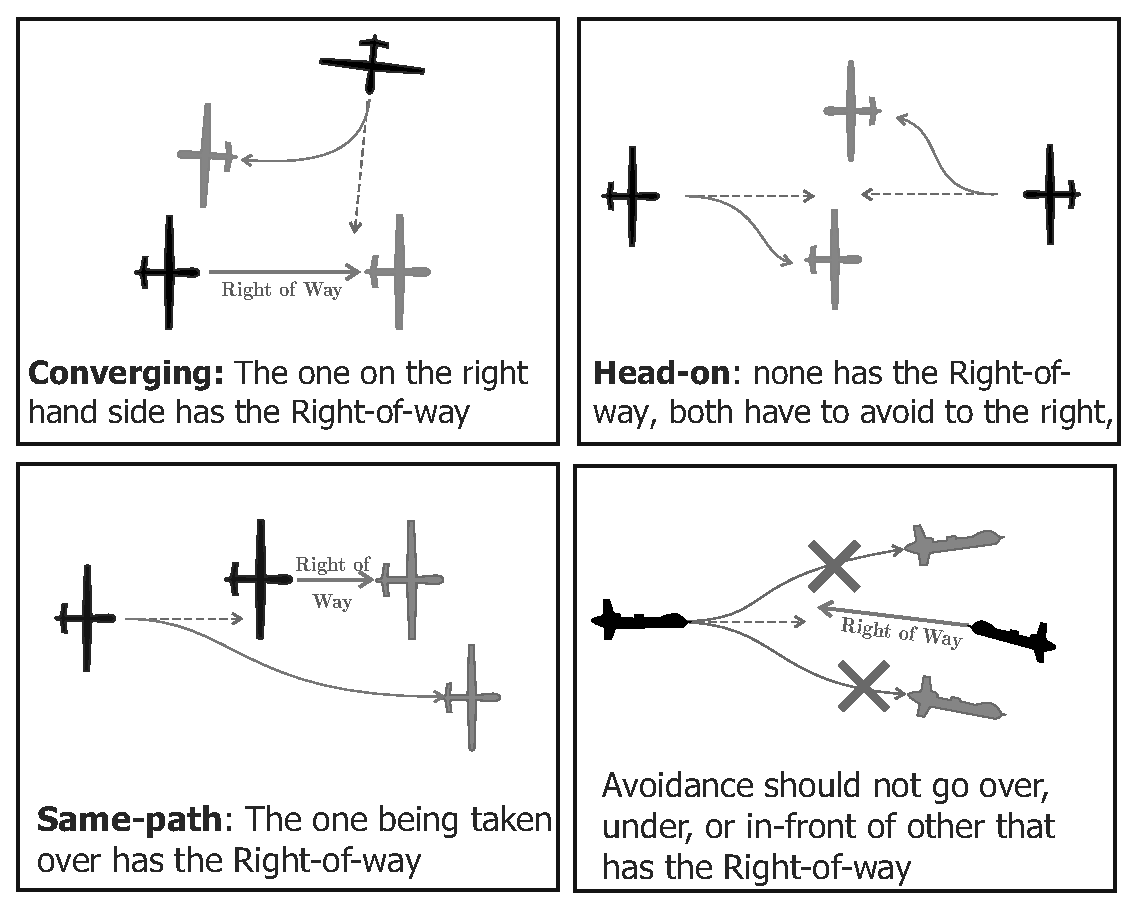
\includegraphics[width=8cm]{\TheDir Figures/RulesPict}
 \caption{The right-of-way rules definitions, adapted from Ref.\cite{FAR:91}}
 \label{f:RulesPict}
\end{figure}

Thus, there are five ways an own-ship can encounter an obstacle, i.e., right-converging, left-converging, head-on, taking-over, or being taken over. The first and the last will make an own-ship obtain the right-of-way (\textbf{\textit{RoW}}), while others will make it lose the right-of-way (\textbf{\textit{$\sim$RoW}}). The type of encounter can be determined by checking the inclusion of the $VO_{oi}$ origin in one of the five additional sets, shown in figure~\ref{f:SVOconcept}-b. The four sectors, $S_{R1}$, $S_{R2}$, $S_{R3}$, and $S_{R4}$, are generated with regard to the own-ship's track, the $X_w- Y_w $ axis, with offsets taken from Ref.~\cite{FARJO:7110}, as shown in figure~\ref{f:SVOconcept}-a. The last set, the $S_{V_o}$, is a circle with radius of $|V_o|$. Lemma 1 elaborates how these sets are used.

\begin{figure}
\begin{subfigmatrix}{1}
\subfigure[]{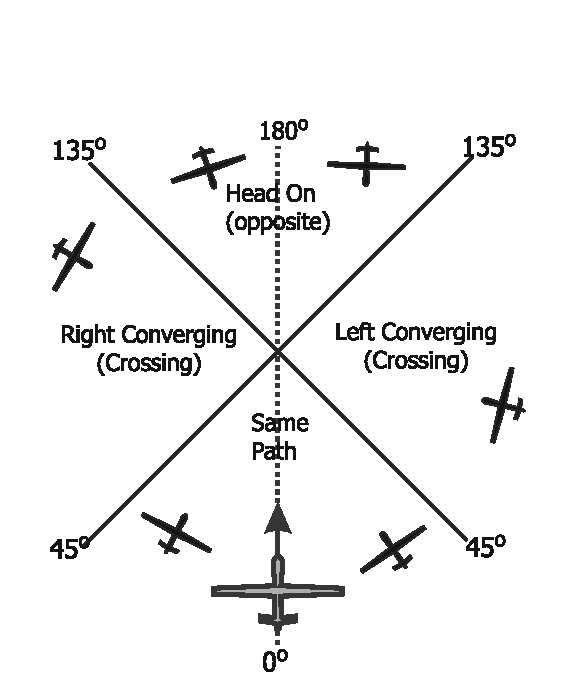
\includegraphics[width=0.45\linewidth]{\TheDir Figures/EncounterDefinitions}}
\subfigure[]{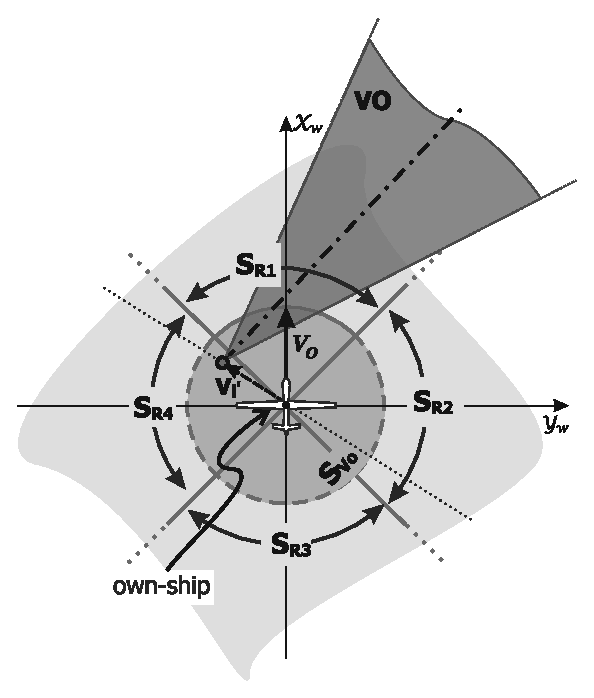
\includegraphics[width=0.45\linewidth]{\TheDir Figures/SVOexpl}}
\end{subfigmatrix}
 \caption{(a) Encounter type definitions, adopted from Ref.\cite{FARJO:7110} (b) SVO additional set definitions}
 \label{f:SVOconcept}
\end{figure}

%THEORY?
\begin{Lemma}
In an encounter situation between the own-ship and an obstacle-$i$, if $V_o \in VO_{oi}$, then,
\begin{enumerate}
\item Whether the own-ship is in a conflict with the obstacle in the same path, converging from left, head-on, or converging from right, can be determined by the inclusion of the origin point of $VO_{oi}$, or the $V_i' $, within the set of $S_{R1}$, $S_{R2}$, $S_{R3}$, or $S_{R4}$, respectively.
\item In case of $V_i' \in S_{R1}$, whether the obstacle is taking-over or being taken-over by the own-ship can be determined by the inclusion or exclusion of the origin point of $VO_{oi}$ from the $S_{V_o}$ set.
\end{enumerate}
\end{Lemma}
%prove?
Ambiguous situations might occur if the $V_i'$ lies exactly on an edge between sets. Hence, a convention is used that determines the types in the following order of priority: head-on, converging, and same-path. 

\subsection{Avoidance Algorithm and the Minimum Avoidance Turning-rate}
Different from previous variations of the VO-method, the SVO algorithm uses three modes to generate the maneuver, i.e., turn, maintain, and mission, as shown in figure~\ref{f:StateFlow}. The turn-mode is set to comply with the right-of-way rules that prefer lateral avoidance to the right and, for simplification, it is limited to turn only without speed alteration. In this mode, the $V_o$ is updated by applying the avoidance-turning-rate, $\omega_{avo}$, instead of point-to-point discrete updates used in the previous VO-methods. The maintain-mode is introduced to keep the own-ship at its current velocity when it has the right-of-way or when $V_o \notin VO_{oi}$ even though the encounter is imminent. This mode is especially used to suppress the oscillation problem in OVO\cite{Snape:11}, that is, when the $V_o$ changes frequently, going back and forth to outside and inside the $VO_{oi}$. The mission-mode is activated when the conflict is cleared, directing the vehicle back to the original goal. The state of the vehicle is initiated also from this mode.

\begin{figure}[h!]
\centering
\includegraphics[width=5cm]{\TheDir Figures/SVOStateflow}
 \caption{State diagram of the Selective Velocity Obstacle algorithm}
 \label{f:StateFlow}
\end{figure}

Two parameters that need to be defined for the algorithm to work are the avoidance distance, $d_{avo}$, and the avoidance-turning-rate, $\omega_{avo}$. To model the heterogeneous situation, each involved vehicle can freely choose their own preference for those parameters. The minimum limit of $\omega_{avo}$ is defined in order to ensure safety. Denoted as $\omega_{a.min}$, the minimum limit of the avoidance-turning-rate is a function of the variables of the encounter-geometry. In the SVO method framework, the geometry includes the speeds ($|V_o|$, $|V_i|$), the initial headings ($\psi_o$, $\psi_i$), and the avoidance starting point ($d_{avo}$), as shown in figure~\ref{f:Grazing}. The kinematic equations for the own-ship, by setting the obstacle relative position as the fixed origin, are described in the relative velocity $V_{R_x}(t)$ and $V_{R_y}(t)$, and their integrals within an interval of time, $X_R(t)$ and $Y_R(t)$, in equation (\ref{eq:XY01a}) and (\ref{eq:XY01b}) .

\begin{figure}
	\centering
	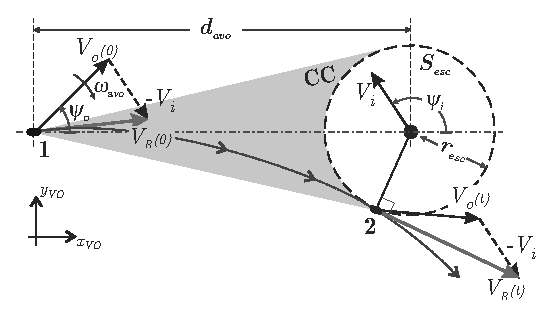
\includegraphics[width=0.8\linewidth]{\TheDir Figures/Grazing}
	\caption{An example of a deconflict maneuver with minimum avoidance turning rate.}
	\label{f:Grazing}
\end{figure}

\begin{equation}
	\label{eq:XY01a}
	\begin{array}{l}
		V_{R_x}(t) = \left| {V_o} \right|\cos \left( {\psi_o+\omega _{avo} t} \right) - {\left| {V_i } \right|} \cos \left( \psi_i \right)\\ 
		V_{R_y}(t) = \left| {V_o } \right| \sin \left( {\psi_o+\omega _{avo} t} \right) - {\left| {V_i } \right|} \sin \left( \psi_i \right)\\ 
	\end{array}
\end{equation}

\begin{equation}
\label{eq:XY01b}
\begin{array}{l}
x_R(t) = \frac{{\left| {V_o } \right|}}{{\omega _{avo} }}\sin \left( {\psi_o+\omega _{avo} t} \right) - {\left| {V_i } \right|} t \cos \left( \psi_i \right)-d_{avo}\\ 
y_R(t) = - \frac{{\left| {V_o } \right|}}{{\omega _{avo} }}\cos \left( {\psi_o+\omega _{avo} t} \right) - {\left| {V_i } \right|} t \sin \left( \psi_i \right)\\ 
\end{array}
\end{equation}

Applying a turning rate, $\omega_{avo}$, from $t=0$, or point-1 in figure~\ref{f:Grazing}, will change the direction of $V_o$, without changing the $V_i$. It can be observed that the own-ship is using the minimum turning rate $\omega_{a.min}$, if it avoids by grazing the edge of the $S_{esc}$, as shown at point-2 in the figure. The boundary conditions for this kind of avoidance are described in equation (\ref{eq:XY02}) and (\ref{eq:XY03}). The former is the relative distance that should be equal to the $r_{esc}$. The latter describes the grazing situation in which the vector of the relative velocity is equal to the tangent line of $S_{esc}$ at the point where the owns-ship touches. Hence, the vector of the relative velocity should be perpendicular to the line from the origin to point-2. 

\begin{equation}
	\label{eq:XY02}
	\sqrt{ {x_R(t)} ^2  +  {y_R(t)} ^2}  = r_{sep} \\ 
\end{equation}

\begin{equation}
\label{eq:XY03}
\left| \frac{V_{Ry}(t)}{V_{Rx}(t)} \right|  = \left|  -\frac{x_R(t)}{y_R(t)} \right|  \\ 
\end{equation}

In this paper, $\omega_{a.min}$ is derived by iterating the value of $\omega_{avo}$ in the relative position equation (\ref{eq:XY01b}), with a random sample of the initial conditions $|V_o|$, $|V_i|$, $\psi_o$, $\psi_i$, and $d_{avo}$. Starting with a small value of $\omega_{avo} =0.01$ degrees/second, the relative positions are solved discretely from $t_0 = 0$, until the own-ship violates the $S_{esc}$ or until the right side of equation (\ref{eq:XY03}) is greater than the left. The process is repeated with increased value of $\omega_{avo}$ by 0.01 degrees/second. The iteration continues until no violation occurs when equation (\ref{eq:XY03}) is fulfilled. Hence the $\omega_{avo}$ at the end of the iteration is the minimum turning rate, $\omega_{a.min}$, for the particular sample.

The $\omega_{a.min}$ value is derived in this research for a thousand randomly selected sets of conflicting initial conditions, ranging in speed from 8 to 13 meters/second, and in avoidance distance from 50 to 700 meters. These are the ranges for UAVs in category I, the Small-slow UAVs, described in Ref.\cite{Jenie:13a}. Figure~\ref{f:ReqTurnRate} maps these results along the corresponding $d_{avo}$. The map shows a clear boundary of the safe $\omega_{a.min}$ for any encounter geometry at a particular $d_{avo}$. This boundary is defined as the recommended minimum turning rate, denoted in this paper as $\omega_{a.min}^*$. It should be noted that different ranges of initial conditions will result in different maps of $\omega_{avo}$ and $\omega_{avo}^*$. 


\begin{figure}
 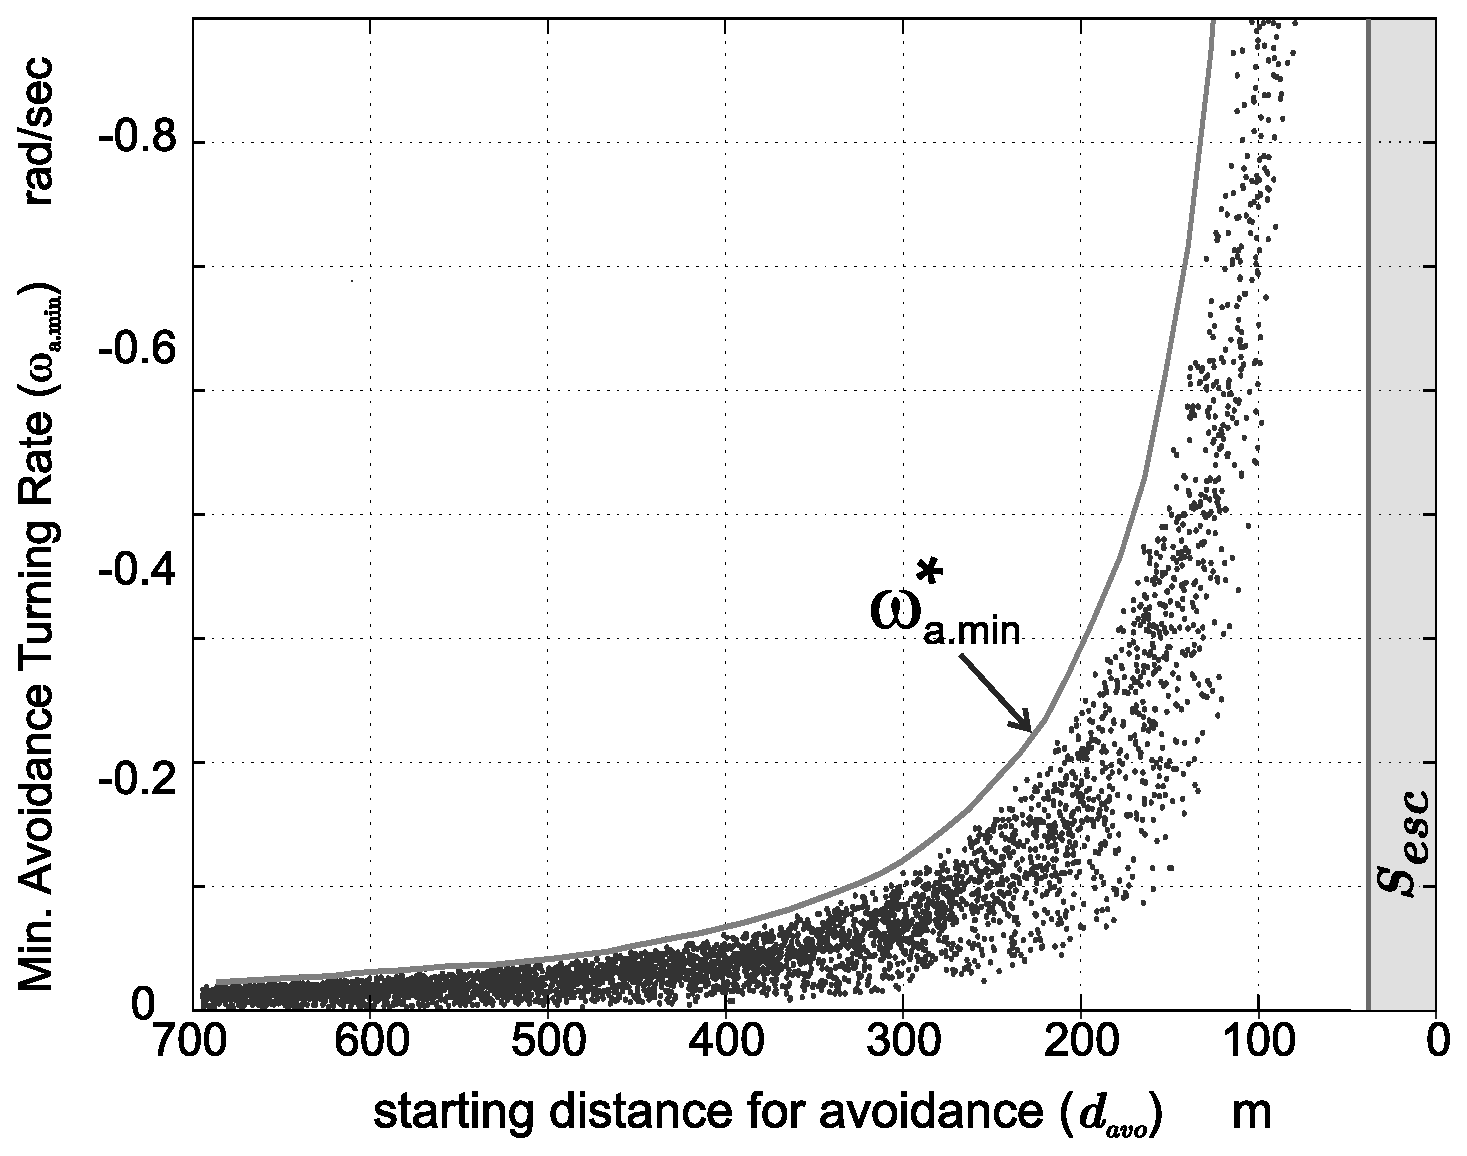
\includegraphics[width=1\linewidth]{\TheDir Figures/MCingRTR}
 \centering
 \caption{Map of $\omega_{a.min}$ from sets of initial conditions, along the corresponding $d_{avo}$}
 \label{f:ReqTurnRate}
\end{figure}


\section{Implementation}
To evaluate the SVO method, a MATLAB program has been developed. It simulates multiple vehicles, each embedded with an avoidance system that is based on the SVO-method algorithm. The simulated vehicles are assumed to exchange their flight-data among each other, such as by using the Automatic Dependent Surveillance Broadcast (ADS-B), without delays or losses. The simulation limits both conflict and motion of the vehicle in the 2-dimensional plane.

\subsection{Simulation Setup}
The simulation presented in this section shows encounters of UAVs from category I; the Small-slow UAVs, which is based on the work in Ref.~\cite{Jenie:13a}. The value of speeds, turning rates and distances to start avoidance, are randomized within the ranges specified in table~\ref{t:RangeSSUAV}. The avoidance maneuver thus starts at an arbitrary point of $d_{avo}$, which is within the deconflicting-zone, 50 to 700 meters from the obstacle. The objective of the avoidance is to prevent violation into the escape-zone $S_{esc}$, which is a circle of radius $r_{esc} = 50$ meters centered on the obstacle.

\begin{table}
 \begin{center}
   \caption{Ranges of parameters for UAVs in category I (Small-Slow UAV)\cite{Jenie:13a}.}
   \label{t:RangeSSUAV}
   \begin{tabular}{lcc}
   \hline \hline
    Parameter & Range & Unit \\
    \hline
    Speed, $|V|$ & 8 - 13 & [ m/s ] \\
    Turning rates, $\omega_{avo}$ &  $\omega_{a.min}^*$ - 5   & [deg/s]\\
    Distance to avoid & 50 -700 & [m] \\
     \hline \hline
   \end{tabular}
 \end{center}
\end{table}

Simulations are conducted for the converging, head-on, and same-path encounters. In all cases, the initial parameters are varied randomly within the ranges listed in table~\ref{t:RangeSSUAV}. The results are presented using time-captures from a top-down point-of-view, as shown in figure~\ref{f:Converge_a} and figures~\ref{f:Converge_b} - \ref{f:TakeOver_ab}. Each circle in those figures represents the half-radius of the $S_{esc}$. The used half-radius for the circle conserves the visualization of the separation, such that when two circles touch, the vehicles are on the edge of each other's escape-zone. 

\subsection{Results}
Figure~\ref{f:Converge_a} depicts a simple converging case of two homogeneous agents. This first simulation shows a deconflict maneuver from a randomly chosen starting point, by applying an avoidance-turning-rate of $5$ degrees/second, well above the $\omega_{a.min}^*$ recommended for that distance (refer to figure~\ref{f:ReqTurnRate}). Figure~\ref{f:TrackComp} shows the comparison of avoidance path profiles between three values of $\omega_{avo}$, i.e., $5^o/s$, the recommended minimum avoidance turning rate $\omega_{a.min}^*=1.71^o/s$, and the true minimum avoidance turning rate $\omega_{a.min} = 0.292^o/s$. The path profiles for using OVO with $\omega_{avo} = 5^o/s$ is shown as well for comparison.  Figure~\ref{f:DistanceComp} shows the comparison of the distance between vehicles showing that the deviation and the CPA are reduced as the turning rate gets slower. The use of the $\omega_{a.min} = 0.292^o/s$, specifically derived for the initial condition of the case, results in the subtlest deconflict maneuver in SVO, resulting zero distance of CPA. The short maintain-mode line in the heading profile in figure~\ref{f:HeadingComp} indicates that the $V_o$ escapes the $VO_{oi}$ set only at the last moment before violation. The fact that this line is not zero, however, indicates a delay in restoring to the mission-mode.

\begin{figure}[h!]
	\centering
	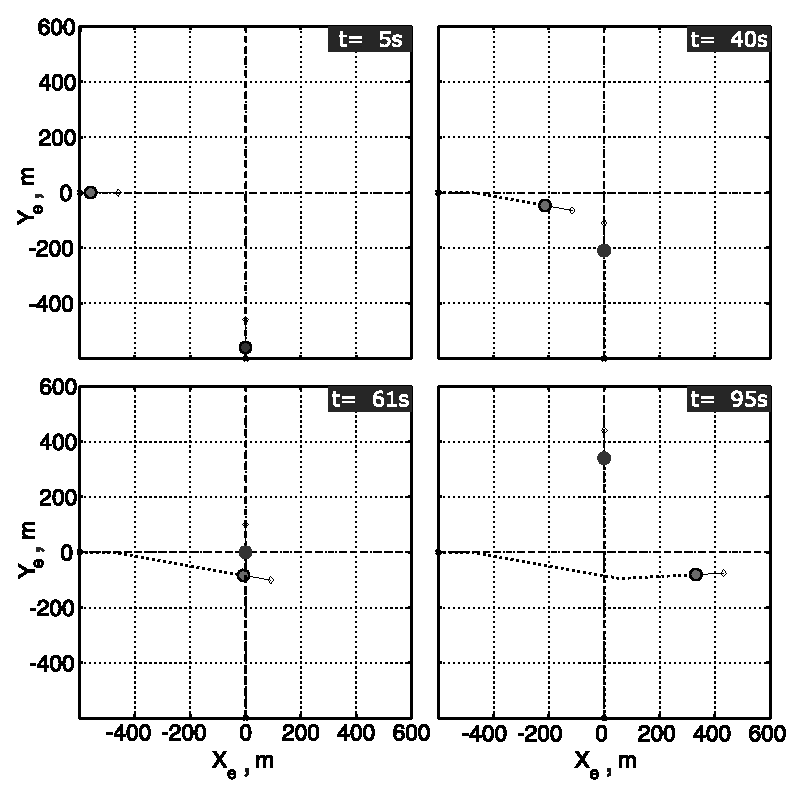
\includegraphics[width=0.8\linewidth]{\TheDir Figures/Converge_2}
	\caption{Simulation of converging encounters and the avoidance solutions using SVO}
	\label{f:Converge_a}
\end{figure}

\begin{figure}[h!]
	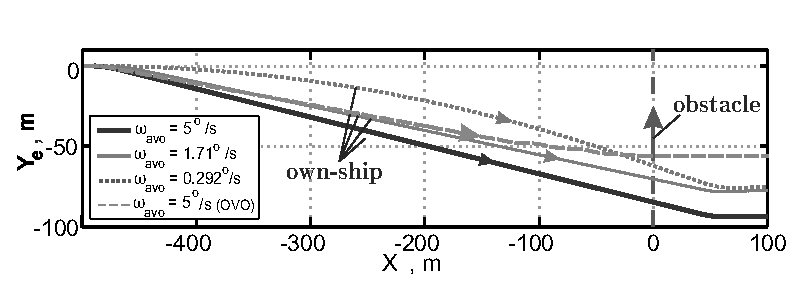
\includegraphics[width=1\linewidth]{\TheDir Figures/TrackComp}
	\centering
	\caption{Comparison of deconflict paths resulting from different $\omega_{avo}$, for the case shown in Figure~\ref{f:Converge_a}.}
	\label{f:TrackComp}
\end{figure} 

\begin{figure}[h!]
	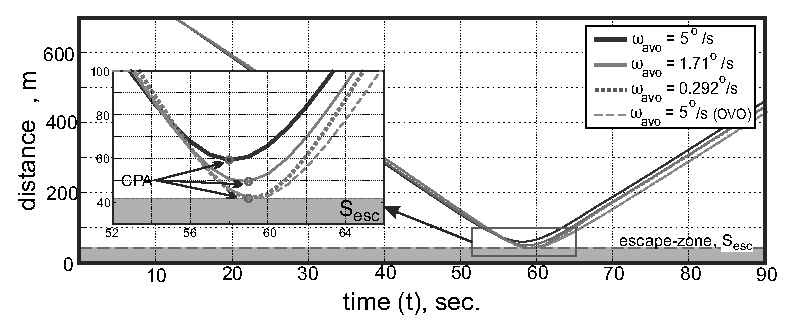
\includegraphics[width=1\linewidth]{\TheDir Figures/DistanceComp}
	\centering
	\caption{Comparison of distances between the pair of vehicles resulting from different $\omega_{avo}$, for the case shown in Figure~\ref{f:Converge_a}.}
	\label{f:DistanceComp}
\end{figure} 

\begin{figure}[h!]
	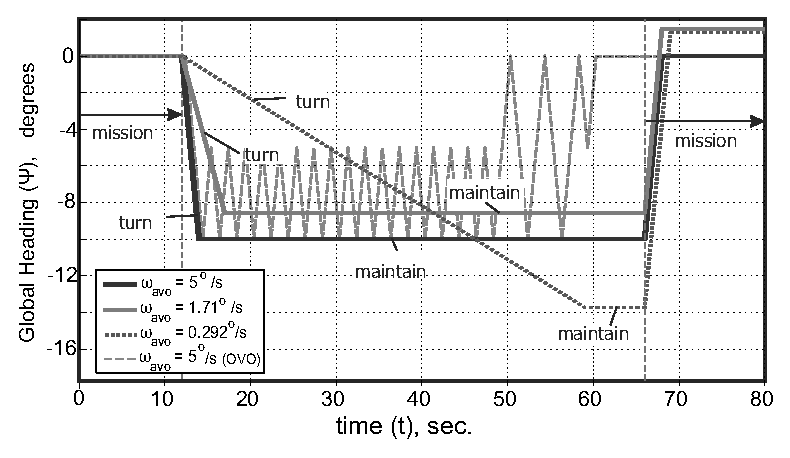
\includegraphics[width=1\linewidth]{\TheDir Figures/HeadingComp}
	\centering
	\caption{Comparison of Heading time-responses resulting from different $\omega_{avo}$, for the case shown in Figure~\ref{f:Converge_a}.}
	\label{f:HeadingComp}
\end{figure}

Figure~\ref{f:TrackComp}, \ref{f:DistanceComp}, and \ref{f:HeadingComp} also show the results of using OVO with $\omega_{avo} = 5^o/s$. The $V_o$ tendency to oscillate in OVO is shown clearly in figure~\ref{f:HeadingComp}, which affected the path of the own-ship. This oscillation can enforced large avoidance turning rate to avoid with zero distance of CPA, but the avoidance will be inefficient since the heading changes frequently. Figure~\ref{f:TrackComp} shows that the SVO can almost match the flight path of OVO using $\omega_{a.min}^*$, without any oscillation. The total path deviation using SVO, however, is larger since the own-ship has to wait in maintain-mode for a while for extra safety, that is, until the $V_o$ is diverging or until the encounter is not imminent anymore.  

Figure~\ref{f:Converge_b} shows a case of heterogeneous multiple encounters. The use of SVO results in different magnitudes of deviation from the corresponding original path. Two of the vehicles even stay exactly on their original path. This simulation also shows the problem with delay in switching to mission-mode in the algorithm that keeps vehicles from restoring their path, even after the CPA is passed. This problem comes from the definition of the $DIV_{oi}$ set, which collects diverging velocities from the entire obstacle flight-path, including the part that has been passed. For instance, as shown in figure~\ref{f:Converge_b}, the last path $A_5$ has to cross belongs to $A_7$, instead of $A_8$, the last vehicle it cleared. Redefinition of the diverging set is required to eliminate this problem. 

\begin{figure}[h!]
	\centering
	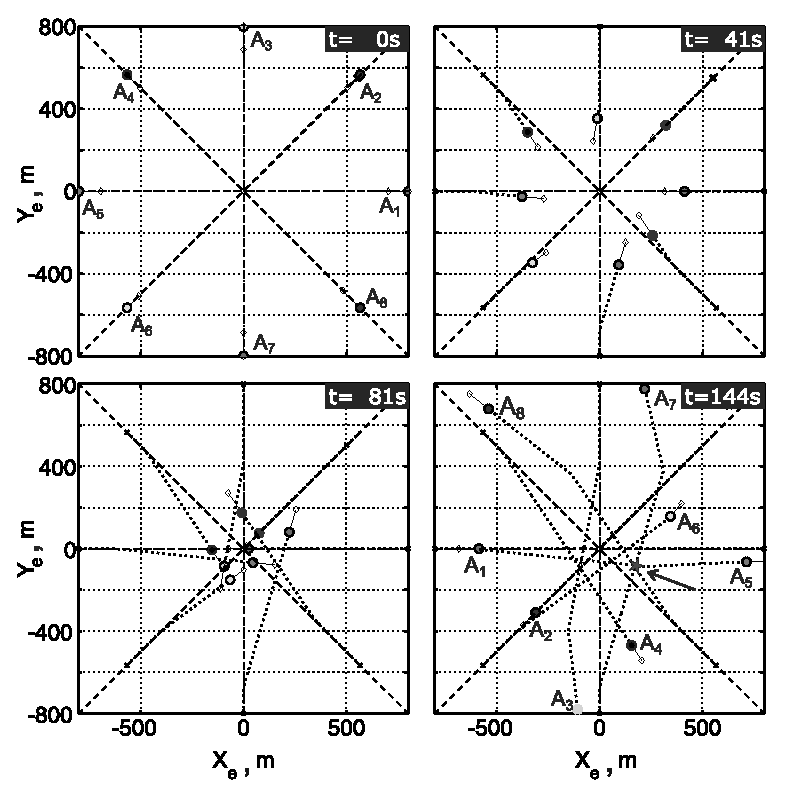
\includegraphics[width=1\linewidth]{\TheDir Figures/Converge_8flex}
	\caption{Simulation of converging encounters and the avoidance solutions using SVO}
	\label{f:Converge_b}
\end{figure}


Figure~\ref{f:HeadOn_ab} and~\ref{f:TakeOver_ab} also show successful deconflict maneuvers in head-on and same-path encounters. The entire avoidance maneuver complies with the right-of-way rules. The result in figure~\ref{f:HeadOn_ab} reveals that multiple head-on encounters will always be mixed with same-path encounters, since the vehicles on the right side are in a same-path situation first. In this case, $A_3$ tries to take over $A_2$ first before it starts to avoid $A_1$. $A_2$ tries to avoid a head-on collision with $A_1$ early, while $A_4$ waits until almost the last moment. $A_4$ deviation becomes large since it has to avoid $A_3$ as well, before it can restore its path.


\begin{figure}[h!]
\centering
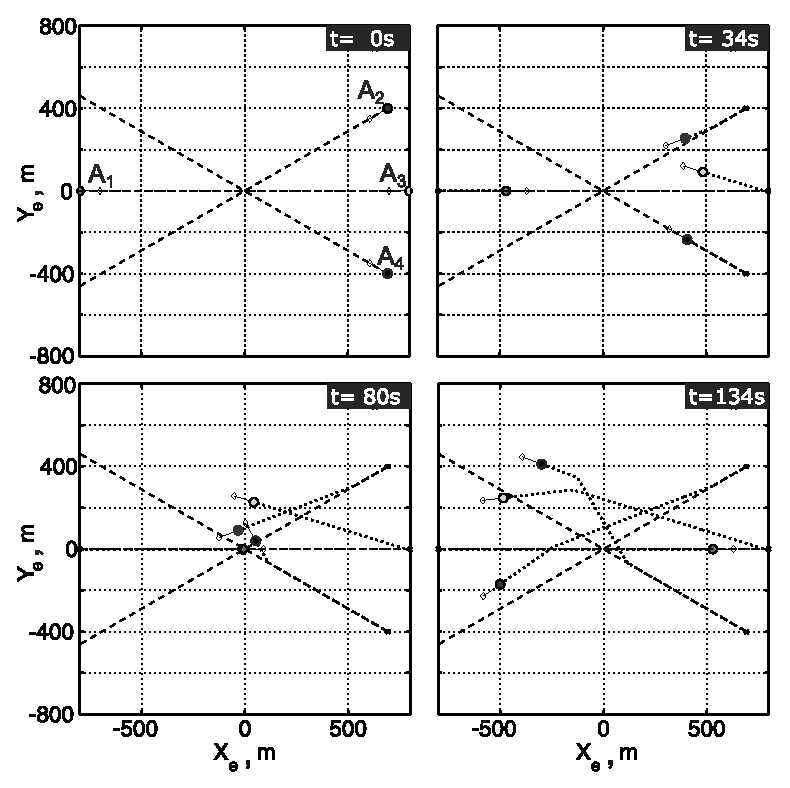
\includegraphics[width=8cm]{\TheDir Figures/HeadOn_4flex}
 \caption{Simulation of head-on encounters and the avoidance solutions using SVO}
 \label{f:HeadOn_ab}
\end{figure}

%fig 9
\begin{figure}[h!]
\centering
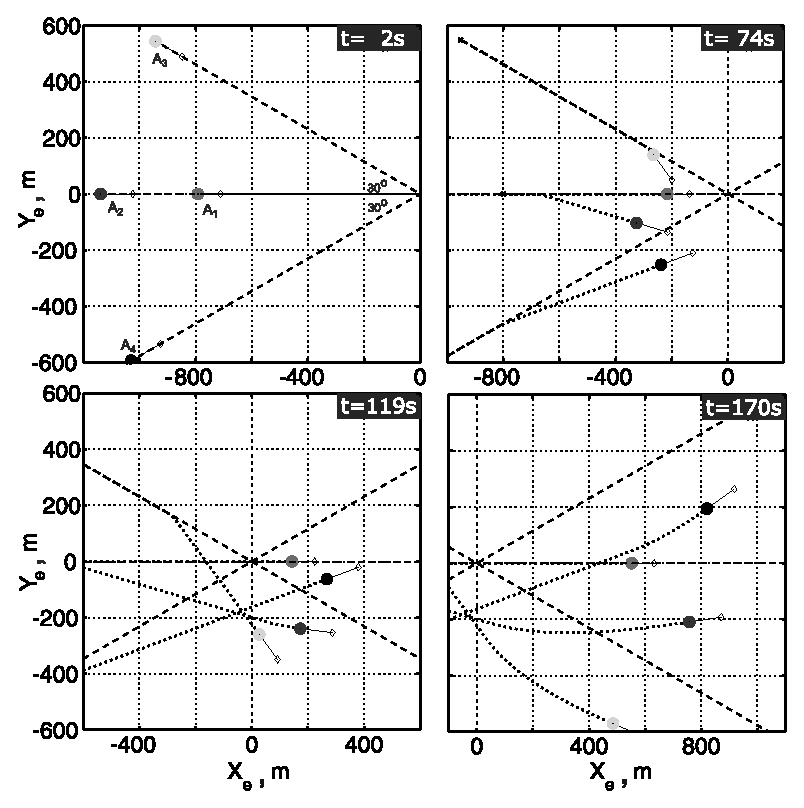
\includegraphics[width=8cm]{\TheDir Figures/TakeOver_4flex}
 \caption{Simulation of same-path encounters and the avoidance solutions using SVO}
 \label{f:TakeOver_ab}
\end{figure}

\subsection{Validation}
The SVO-method is validated using Monte Carlo simulations with random initial condition setup across the simulation, within the ranges specified in table~\ref{t:RangeSSUAV}. The simulations involve two to five vehicles that are randomly directed and positioned. Initially, all vehicles are positioned outside each other's deconflict-zone, within a square area that is proportional to the number of vehicles, i.e., $(N\times 1000)^2$ meter-square. These random scenario generations act as replacements for the lack of operational data and models, the two sources of scenarios that are commonly used in TCAS validation\cite{kochenderfer:2012}. The violation probability, $P_{vio}$, is defined in equation~(\ref{eq:Pvio1}), i.e.,

\begin{equation}
\label{eq:Pvio1}
{P_{vio}} = \frac{{{N_{vio}}}}{{{N_{MC}}}}
\end{equation}

The $N_{vio}$ is the number of violation occurred and $N_{MC}$ is the number of the total Monte Carlo samples, which is at least $10^6$ samples. For comparison, this probability is derived for cases without avoidance, with OVO avoidance, and with SVO avoidance, as shown in table~\ref{t:ProbResult}. The OVO in this case uses a large turning rate of $5^o/s$ with a randomly generated direction, i.e., to the left or to the right.

From the result for cases without any avoidance, it can be concluded that the probability of conflict will always exist and gets higher with the number of vehicles involved, even if the area of interest is widened proportionally. The OVO is able to suppress the number of violations into almost one-hundred time smaller. Some failed avoidances, however, still occur mainly contributed to the oscillation and the reciprocating dance problem\cite{Snape:11}. The SVO is demonstrated to be able to resolve conflicts and avoidance problems, with zero violations in all samples of initial condition. 

An interesting note is that all the conflicts across the samples are pairwise, i.e., only between two vehicles. In fact, it is hard to find a multiple-encounter situation, such as shown in figure~\ref{f:Converge_b}, in a random setup, which suggest that the SVO only needs to resolve conflicts in a one-by-one manner. Therefore, the validation result is limited to single-encounters. Further analysis is required to determine the SVO validity in more stressful multiple-encounter condition.   

\begin{table}[h!]
 \begin{center}

   \caption{Violation probability in cases without avoidance, using the OVO, and using the SVO.}
   \label{t:ProbResult}
   \begin{tabular}{cccc}
   \hline \hline
    Number of Vehicles & \multicolumn{3}{c}{Probability of Violation}\\
     & No Avoidance &  Using OVO\tnote{\dag} & Using SVO \\
    \hline
    2 & 1.033 \% & 0.01  \% & 0 \% \\
    3 & 2.366 \% & 0.029 \% & 0 \% \\
    4 & 3.838 \% & 0.046 \% & 0 \% \\
    5 & 5.353 \% & 0.056 \% & 0 \% \\
     \hline \hline
   \end{tabular}
%   \begin{tablenotes}
%   	\item[\dag] Using randomly generated direction of avoidance, with $\left| \omega_{avo} \right| = 5^o/s$,
%   \end{tablenotes}
 \end{center}
\end{table}

\section{Conclusion}
This paper elaborates the novel Selective Velocity Obstacle Method (SVO) that supports Unmanned Aerial Vehicle (UAV) autonomous collision avoidance. The SVO is shown to be able to generate deconflict maneuvers separately to resolve heterogeneous situations, while obeying the right-of-way rules, using a distance-based prescribed turning rate. Problems in the original Velocity Obstacle method (OVO) are resolved in SVO and validated trough a Monte Carlo simulations procedure. The procedure also reveals that, in a random situation setup, multiple-encounters are very unlikely to happen and, hence, the SVO only needs to resolve conflicts in one-by-one manner. Several challenges in the method are noted, such as the late onset in restoring to the mission-mode. The method also does not consider a wide range of vehicle types, possible uncertainties in the exchanged data, and three-dimensional conflicts. The results, however, show that the SVO is a suitable method to reduce the risk of collision and, hence, increase the safety of UAV operations in the airspace system.
